\chapter{Methods}\label{cha:methods}

\section{Overview}

In this section, I first introduce fundamental geometric considerations which inform the derivation and implementation of each subsequent method (Section~\ref{sec:considerations}).

Next, I outline a method for measuring surface \emph{attitude} data via topography and the orientation of discordant lava flow features (Section~\ref{sec:mapping}). While this dataset alone provides evidence of surface deformation \parencite[c.f.][]{mouginis-mark_late-stage_2019}, I show that it is insufficient for physically quantifying this deformation, i.e., estimating reservoir location (horizontal and vertical), volume, pressure change, etc. I also briefly discuss some limitations and necessary assumptions of this method. 

Before describing a solution to this problem, it is necessary to introduce a method for gathering modelled \emph{displacement} data corresponding to Olympus Mons' elastic response to reservoir pressure change. I use this method to explore a wide space of model parameters including gravitational loading, paleo-topography, and magma reservoir depth, size, shape, and pressure change. Once again, I discuss limitations and criteria for assessing physical plausibility of these models.

Finally, I develop a geometric framework to directly compare mapped attitude data and modelled displacement data. Key steps in this framework include:
\begin{enumerate}
    \item Letting the assumption of axisymmetry impose a unique solution to the under-determined discordance problem. Specifically, a given pair of points---one axisymmetric inflation center and one sample with incomplete attitude data---is sufficient to complete the attitude dataset for that point and calculate tilt.
    \item Converting displacement data along an axisymmetric model surface into tilt. While this method is not used immediately, it sets up an important derivation: a simplified analytical solution providing tilt as a function of distance with two parameters linked to the physical characteristics of the underlying reservoir pressure change.
    \item Evaluating the degree to which axisymmetric ``epicenter'' (map-view location) candidates can explain observed topographic discordance under the assumption of axisymmetric pressure change. For each center candidate, this involves determining the unique\footnote{if it exists at all.} tilt solution for each sampled point as a function of distance from that center, then fitting the general analytical tilt function to the resulting dataset (or sub-populations thereof). Each center is then evaluated on the goodness of fit and physical plausibility of these parameters, among other criteria.
\end{enumerate}

\section{Fundamental Considerations}\label{sec:considerations}

\subsection{Topographic Discordance [REDO FIGURE]}

Numerous lava flows around the summit caldera of Olympus Mons appear to flow uphill~\parencite[Figure~\ref{fig:uphill-flows}; after][]{mouginis-mark_late-stage_2019}. In this thesis, the term \ac{disc} is defined as the angular difference between a lava flow's downhill azimuthal direction and the local dip direction of the underlying surface. For example, a flow pointing directly uphill would have $\acs{disc}=\ang{180}$. 

Discordant lava features have long been used to infer surface deformation under the assumption that lava flows record the downhill direction at the time of their emplacement. This method has been applied at a regional scale to constrain flexural loading of the lithosphere from large volcanic edifices \parencite{mouginis-mark_ancient_1982,isherwood_volcanic_2013,chadwick_late_2015} and more recently to reservoir-scale processes at the summit of Olympus Mons \parencite{mouginis-mark_late-stage_2019}.

The goal of this thesis is to derive as much information as possible from the spatial pattern of topographic discordance at the summit of Olympus Mons. 

\begin{figure}
    \centering
    \includegraphics[width=\textwidth]{uphill-flows.pdf}
    \caption[Discordant lava flows]{Several lava flows (white) in the southern flank region appear to flow uphill toward the modern summit. \acs{CTX} mosaic basemap. Contours in \unit{\km}. After Figure 3 in \textcite{mouginis-mark_late-stage_2019}.}%
    \label{fig:uphill-flows}
\end{figure}

\subsection{Axisymmetry [FINISH TEXT]}

Numerical models are widely used by physical volcanologists to better understand a wide array of observed phenomena in terms of their underlying mechanisms. One advantage of these simulated models (as opposed to physical models involving real materials) is the diversity of conditions available to be tested, from the deep mantle \parencite[e.g.,][]{redmond_numerical_2004,ogawa_four-stage_2021} or volcanic edifices and their surroundings \parencite[e.g.,][]{isherwood_volcanic_2013} to individual magma reservoirs \parencite[e.g.,][]{grosfils_magma_2007,grosfils_elastic_2015}. Many of these models are axisymmetric, reflecting the common characteristic that many volcanic and magmatic features are roughly circular in plan view. While this sacrifice the ability to assess certain asymmetric features, they are much easier to construct, take much less time to run due to the massively simplified geometry, and often capture major characteristics of the system in question.

\begin{figure}
    \begin{tikzpicture}[scale=1.5,tdplot_main_coords]

% origin
\coordinate (orig) at (0,0,0);
\coordinate (summit) at (0,0,2.5);

\coordinate (bottomcorner) at (0,3*\radius,0);
\coordinate (topcorner) at (0,3*\radius,1);
\coordinate (topcorneropp) at (0,-3*\radius,1);
\coordinate (foot) at (0,\radius,1);
\coordinate (footopp) at (0,-\radius,1);

\coordinate (arrow) at (0,1.5*\radius,.5);
\coordinate (arrowopp) at (0,-1.5*\radius,.5);

% also defines (Pxy), (Pxz), (Pyz), etc.
\tdplotsetcoord{P}{\radius}{\ze}{\az}

% draw bottom surface
\draw (0,0,0) circle (3*\radius);
\fill[opacity=0.05] (0,0,0) circle (3*\radius);

% back half line
\draw[red,arrow] (arrow) arc (90:450:1.5*\radius);
\draw (foot) arc (90:450:\radius);

% back half fill
\foreach \y in {90,...,269}{
    \fill[opacity=0.05] (\y:\radius) + (0,0,1) arc (\y:\y+1:\radius) -- (summit);
    \fill[opacity=0.05] (\y:3*\radius) -- (\y+1:3*\radius) --+ (0,0,1) arc (\y-360:\y-361:3*\radius);
};

\fill[opacity = 0.05] (topcorner) arc (90:270:3*\radius);

% cross section
\fill[white] (orig) -- (summit) -- (foot) -- (topcorner) -- (bottomcorner);
\draw (orig) -- (summit) -- (foot) -- (topcorner) -- (bottomcorner) -- (orig);

% axes
\draw[axis] (orig) -- (0,0,2*\axislength) node[anchor=south]{$z$};
\draw[axis] (orig) -- (0,3*\axislength,0) node[anchor=west]{$r$};

% front line
\draw[red,arrow] (arrowopp) arc (270:450:1.5*\radius);
\draw (footopp) arc (270:450:\radius);

% front fill
\foreach \z in {270,...,449}{
    \fill[opacity=0.05] (\z:\radius) + (0,0,1) arc (\z:\z+1:\radius) -- (summit);
    \fill[opacity=0.05] (\z:3*\radius) -- (\z+1:3*\radius) --+ (0,0,1) arc (\z-360:\z-361:3*\radius);
};

\fill[opacity = 0.05] (topcorneropp) arc (270:450:3*\radius);

% draw middle surfaces
\draw (0,0,1) circle (3*\radius);

\end{tikzpicture}%
    \caption[Axisymmetry]{Schematic illustration of an axisymmetric model. A 3D feature with rotational symmetry about a vertical axis is fully described by a single cross-section (white). Conceptually this surface can be swept around the axis of symmetry (red arrow) to reconstruct the 3D shape. Radial $(r)$ and vertical $(z)$ coordinates describe position within the model.}%
    \label{fig:axisymmetry}
\end{figure}    

In this thesis, I seek to compare surface tilt inferred at the summit with tilt resulting from pressure changes in an underlying magma reservoir. Since this thesis is an early component of a larger research program to assess late Amazonian magmatism at Olympus Mons, I use the simplified\footnote{I justify additional simplifying assumptions in Section~\ref{sec:modelling}.} axisymmetric condition in my numerical models. Therefore, I make the same assumption when estimating tilt from discordant lava flows at the summit.

\subsection{Attitude Data Representation [FINISH TEXT AND FIGURE]}

The data I collect, calculate, and analyze in this thesis refer to attitude: the 3D orientation (primarily of surfaces) in space. It is important to use a suitable and consistent graphical representation of these data. The most common such representation in geology is the lower-hemisphere stereographic projection, in which linear and planar features are represented by their intersections with a unit sphere whose center lies within the feature.

In this thesis, I use an orthographic (rather than stereographic) projection of this same sphere. Rather than projecting from a point on the sphere, features are projected perpendicular to the map surface. The reason for this change is that small circles whose axis is on the primitive circle project to straight lines, which is most convenient for the derivation in Section~\ref{sec:paleo-slope} and elsewhere.

Additionally, planes are often plotted by their curvilinear intersection to help set them apart from linear features, whose intersections are points. However, I do not describe any linear attitudes in this thesis, and curvilinear intersections quickly become unwieldy. Therefore, I define all planes by their poles, or the unique linear attitude normal to any plane.

Additionally, the projection I use is of the upper hemisphere, not the lower hemisphere.

\begin{figure}
    \begin{tikzpicture}[scale=4.4,tdplot_main_coords]

% origin
\coordinate (O) at (0,0,0);

% also defines (Pxy), (Pxz), (Pyz), etc.
\tdplotsetcoord{P}{\radius}{\ze}{\az}

% fill flat surface
\fill[color = gray!10!white] (0,0) circle (0.5*\radius);

% define tilted surface
\tdplotsetrotatedcoords{\az}{\ze}{0}

% fill tilted surface
\fill[tdplot_rotated_coords, color = green!40!black, opacity=0.4] (0,0) circle (0.4*\radius);

% downhill line
\draw[arrow, tdplot_rotated_coords] (0,0) -- (0:0.4*\radius);

% horizontal surface (front right)
\fill[color = gray!10!white, opacity=0.6] (\az:0.5*\radius) arc (\az:\az+90:0.5*\radius) -- (0,0);

% perpendicular corners
\draw[tdplot_rotated_coords] (0.25,0,0) -- (0.25,0,0.25) -- (0,0,0.25) -- (0,-0.25,0.25) -- (0,-0.25,0);

% horizontal surface (front left)
\fill[color = gray!10!white, opacity=0.6] (\az-90:0.5*\radius) arc (\az-90:\az:0.5*\radius) -- (0,0);

% z axis
\draw[axis] (O) -- (0,0,0.5*\axislength) node[anchor=south]{$z$};

% line az surface
\draw[very thin, dashed,green!40!black] (P) -- (Pxy) -- (O);
\draw[arrow, green!40!black] (O) -- (P) node[anchor = south west] {};

% north axis
\draw[axis] (O) -- (0,0.4*\axislength,0) node[anchor=west]{\acs{north}};

% az angle label
\tdplotdrawarc{(O)}{0.4*\radius}{\az}{90}{coordinate, pin={[pin edge={black},-]-60:\acs{az2}}}{}

% az surface
\tdplotsetthetaplanecoords{\az}

% ze angle label
\tdplotdrawarc[tdplot_rotated_coords]{(O)}{0.4*\radius}{0}{\ze}{coordinate, pin={[pin edge={black},-]80:\acs{sl2}}}{}

% ze angle label
\tdplotdrawarc[tdplot_rotated_coords]{(O)}{0.4*\radius}{90}{90+\ze}{coordinate, pin={[pin edge={black},-]180:\acs{sl2}}}{}

\fill[black] (O) circle (0.2pt);

\end{tikzpicture}%
    \caption[Pole to plane]{Pole to Plane in an upper hemisphere orthographic projection.}%
    \label{fig:surface}%
\end{figure}

\section{Mapping Discordant Features}\label{sec:mapping}

\subsection{Preparation of Published Data}

The \acf{CTX}\footnote{aboard the \ac{MRO} spacecraft launched in 2005 by \acs{NASA}.} captures \qty{\sim30}{\km} swaths across the entire martian surface in visible $(\lambda=\qtyrange{500}{800}{\nm})$ greyscale at \qty{\sim6}{\m} spatial resolution. \textcite{Dickson2018AGB} blended these swaths to produce a raster mosaic product (hereafter, ``\ac{CTX} mosaic'') which I use to visually identify and map lava flows and flow channels.

The \acf{MOLA}\footnote{aboard the now-retired \ac{MGS} spacecraft launched in 1996 by \acs{NASA}.} returned topography data with horizontal resolution of \qtyproduct{300 x 1000}{\m} at the equator (better at high latitudes) and elevation uncertainty of \qty{\sim3}{\m}~\parencite{smith_mars_2001}. To improve spatial resolution, additional elevation data from the \ac{HRSC}\footnote{aboard the \ac{MEX} spacecraft launched in 2003 by the \ac{ESA}} was blended to product a \ac{DEM} with \qty{200}{\m} pixel resolution. Each pixel's vertical uncertainty is \qty{\sim1}{\m}, with an additional global uncertainty of \qty{\sim1.8}{\m} in the martian areoid (martian equivalent of Earth's geoid). In this project, the global areoid uncertainty is not a concern because only one region (the summit of Olympus Mons) is considered.

I load these two data sources in an equal-area sinusoidal Mars projection in ArcGIS Pro. The study area is defined by a square \qtyproduct{200 x 200}{\km} centered at the centroid of the outermost \qty{19}{\km} contour,\footnote{This is the highest integer \unit{km} which is roughly circular and completely encloses the caldera complex, implying that it largely records the conical shape of the shield edifice without influence from subsequent caldera collapse or reservoir inflation.} as seen in Figure~\ref{fig:summit}.

\subsection{Study Area Definition \& Preliminary Analysis}

Figure~\ref{fig:summit} shows important topographic patterns at the summit of Olympus Mons. More than \qty{50}{\km} from the center of the figure, topographic contours (\qtyrange{12}{19}{\km}) are fairly regular concentric rings. Closer to the caldera, this axisymmetry breaks down: the caldera complex itself consists of six intersecting collapse pits. On the southern flank, we see a prominent arcuate \qty{20}{\km} contour with the topographic summit (within the \qty{21}{\km} contour) over \qty{20}{\km} from the southern caldera rim. Thus, my first task is to determine the degree to which axisymmetric inflation can apply to an edifice which is not entirely axisymmetric. It is important to point out, however, that the asymmetry inherent to the region is crucial for the discordant flow method to function, as I describe in subsequent sections. 

\subsection{Mapping Lava Features}

I use the \ac{CTX} mosaic to visually identify lava flows near the summit of Olympus Mons. Following \textcite{mouginis-mark_geologic_2021}, I map lobate flow outlines as polygons where possible. From these polygons, I derive centerline features using the \hlss{Polygon To Centerline} tool, as shown in Figure~\ref{fig:flow}.

Where flow margins are not visible, I map channels directly as linear features. I include discontinuous regions where I infer partial collapse of lava tubes yielding skylight chains,\footnote{The assumption of underlying continuity follows, e.g., \textcite{bleacher_olympus_2007,carr_geologic_2010,peters_lava_2021}.} as shown in Figure~\ref{fig:channel}.

\subsection{Paleo-Azimuth from Mapped Features}

I use the \hlss{Calculate Geometry Attributes} tool to find the azimuthal orientation from the start to the end of each feature. This angle is the variable \ac{az1} to each feature, although the following section discussion explains why this variable is not quite ready for use in attitude analysis. While I maintain a consistent ``sense'' in my channel mapping (pointing away from rather than toward the caldera center), the \hlss{Polygon To Centerline} tool does not. Therefore, some flow centerlines need to be reversed using the \hlss{Flip Line} tool.

To determine which centerlines must be reversed, I use the \hlss{Near} tool to determine the azimuth angle from each linear feature to the center of the study area \acs{center}. Here, I leverage my initial observation that all flows in the study area point generally \emph{away} from the caldera center. Therefore, a correctly oriented feature is one where \acs{az1} is \ang{\sim180} away from the calculated angle; at the very least, it should be \ang{90} away. Therefore I select features where this angular difference is less than \ang{90} to reverse using \hlss{Flip Line}, as shown in Figure~\ref{fig:flip-line}. With all features now correctly oriented away from the caldera center, I recalculate the true \ac{az1} value using \hlss{Calculate Geometry Attributes}.

\begin{figure}
    \includegraphics[width=\textwidth]{flip-line.jpeg}%
    \caption{Flip Line}%
    \label{fig:flip-line}
\end{figure}

\subsection{Modern Attitude from Topography}

\newcommand{\samplinginterval}{\qty{3}{\km}}

Along each linear feature, I use the \hlss{Generate Points Along Line} tool sampling interval \samplinginterval\ to create a series of point features where further attitude data collection and analysis will take place. Note that features with length $<\samplinginterval$ are not sampled at all.

\begin{figure}
    \centering
    \begin{subfigure}{\textwidth}
        \centering
        \includegraphics[width=\textwidth]{flow.pdf}
        \caption[Mapped lava flow \& centerline]{A flow with lobate boundaries at each margin is mapped as a polygon (white) from which a linear centerline is derived for sampling.}%
        \label{fig:flow}
    \end{subfigure}
    \begin{subfigure}{\textwidth}
        \centering
        \includegraphics[width=\textwidth]{channel.pdf}
        \caption[Mapped lava channel]{A lava channel is mapped as a linear feature, including regions of discontinuity which are inferred to be collapsed skylight chains over lava tubes.}%
        \label{fig:channel}
    \end{subfigure}
    \caption{Mapping linear features}%
    \label{fig:mapping-linear}
\end{figure}

\begin{figure}
    \centering
    \includegraphics[width=\textwidth]{sampling.pdf}
    \caption[Sampling site selection]{Each linear feature is assigned an average paleo-dip direction. Points are selected for sampling and calculations at \qty{5}{\km} and \qty{3}{\km} intervals for flows and channels, respectively. Paleo-dip direction is assigned to each point from its corresponding line; modern dip and dip direction is assigned to each point from its unique \ac{DEM} neighborhood.}%
    \label{fig:sampling}
\end{figure}

\newcommand{\neighborhood}{\qty{2}{\km}}

The first variable collected is \ac{az1}, which each point inherits from its parent linear feature.

Then, I use the \hlss{Surface Parameters} tool on the \ac{MOLA} \ac{DEM} to compute average topographic \hlss{Slope} and \hlss{Aspect} (downhill azimuth) rasters across the entire study area. To avoid capturing local topographic anomalies, these values are averaged over a ``neighborhood'' with radius \neighborhood. I use the \hlss{Extract Multi Values to Points} tool to assign \ac{sl2} and \ac{az2} to each based on the value of the corresponding raster value at that location. Figure~\ref{fig:tilt-from-map} includes a geometric view of these variables in attitude space alongside \acs{az1}.

\section{Numerically Modelling Reservoir Pressure Change}\label{sec:modelling}

In this section, I model pressure changes (either inflation or deflation) of a magma reservoir under the mapped study area.

I use the numerical modelling software COMSOL Multiphysics 6.1 (COMSOL) to construct a numerical representation of Olympus Mons. The model is axisymmetric, about the center point discussed previously as the center of the \qty{19}{\km} contour.

From this point, elevation transect due south from the study area center point to the base of the edifice \qty{\sim240}{\km} away. This particular center point is derived from the summit of a topographic spline: an interpolation of a hypothetical paleo-topography based on the existing topography outside the \qty{19}{\km} contour (Figure~\ref{fig:summit}). The topography of this outer region \emph{is} roughly axisymmetric and assumed to be relatively unaffected by subsequent caldera and reservoir activity.

I use the \hlss{Parametric Sweep} tool to perform a sequence of analyses which are identical except for specifically controlled parameters: \ac{DtT}, \ac{Rr}, \ac{Rz}, and a \ac{mult}:
\begin{equation}
    \acs{dP}=\acs{mult}\times\acs{rhor}\times\acs{g}\times\acs{DtT},
\end{equation}
where \acs{dP} is the simulated over- (positive) or under-pressure in the reservoir. For each numerical model, I output surface displacement in the radial and vertical direction as a function of distance from the inflation center. 

\subsection{Axisymmetric Elastic Model}

Figure~\ref{fig:axisymmetry} illustrates that the assumption of axisymmetry reduces the 3D edifice to a cross-sectional plane which is equivalent for modelling.

TODO: describe Hookean elasticity assumption.

\subsection{Finite Element Method}

The \ac{FEM} is widely used to model phenomena ranging from fluid flow, heat transfer, and mechanical stress in engineering and geology. This method involves discretizing a continuous medium by constructing a \emph{mesh:} a network of nodes connected to their neighbors by edges. Polygons enclosed by these edges are called elements. Software then solves the chosen equations to compute the variables of interest only for the nodes, whose values can then be interpolated within each element to determine the solution for any point within the continuum.

\section{Synthesis}

The previous sections introduce some broad considerations and describe basic mechanics of data collection methods as they exist in isolation. However, the methods for \emph{analyzing} those data in light of those considerations are difficult to partition into ``mapping'' and ``modelling.'' Therefore, the sequence of methods in this section frequently transitions between map- and model-related data, functions, etc.

To keep this process organized, I bring all data (map-derived attitude and position, model-derived displacement and position) into a Jupyter Notebook environment using the Python programming language (version 3.10.0). Python is an open-source, general purpose language whose large library of modules make it a popular choice for scientific computing applications.

In the body of this section, I describe conceptually and graphically the sequence of computations I would perform for a single analysis. The full source code I use to implement these operations for my entire dataset is included in Appendix~\ref{app:code}.

\subsection{Deriving Tilt from Mapped Attitude Data}

\subsubsection{Spatial Description of Sampled Points}

Mars' rotation about an essentially fixed axis provides a convenient coordinate system of \ac{lat} and \ac{lon} for describing surface position. However, an \emph{axis}ymmetric model imposes a different coordinate system---one defined with respect to the axis of rotational symmetry.

Points mapped in GIS are automatically expressed in \ac{lat} and \ac{lon}; I need to convert this into polar coordinates $(\acs{dist},\acs{bearing})$ with the axisymmetric center as the origin. And because one goal of the project is to evaluate an array of candidate center points, I need an equation that takes any set of center coordinates $(\acs{latC}, \acs{lonC})$ and any set of sample point coordinates and returns a $(\acs{dist},\acs{bearing})$ pair.

To calculate \acf{dist}, I use the spherical law of cosines\footnote{Also known as the great circle distance formula, derived in Appendix~\ref{app:spherical-trig}.} scaled by the martian equatorial radius since Olympus Mons is close to the equator:
\begin{equation}
    \acs{dist}=\arccos(\cos\acs{latC}\cos\acs{lat}\cos(\acs{lonC}-\acs{lon}) + \sin\acs{latC}\sin\acs{lat})\cdot\qty{3396.2}{\km}.
\end{equation}

It turns out that error in the calculated \acs{bearing} value is much more significant than error in \acs{dist}. That's because I use \acs{bearing} to define the axis of tilt and thus the value of tilt for a given center-sample pair, and this computation is very sensitive to minor variations.

Therefore, I make the following choices especially carefully. First, the bearing of a great circle segment is not constant. Since all the calculations take place at the sampled point, I define \acs{bearing} as the geographic azimuth angle directly \emph{away} from \acs{center}. This is to ensure that the horizontal \acs{bearing}-axis points in the same direction as positive \acs{dist}.
\begin{equation}
    \acs{bearing} = \ang{180} + \arctan\left(\frac{\sin(\acs{lonC}-\acs{lon})\cos\acs{latC}} {\cos\acs{lat} \sin\acs{latC}-\sin\acs{lat}\cos\acs{latC}\cos(\acs{lonC}-\acs{lon})}\right).
\end{equation} 

\subsubsection{Paleo-Slope Equation}\label{sec:paleo-slope}

\begin{figure}
\begin{center}
    \begin{tikzpicture}[scale=5,tdplot_main_coords]
    % origin
    \coordinate (orig) at (0,0,0);
    
    % also defines (Pxy), (Pxz), (Pyz), etc.
    \tdplotsetcoord{P}{\radius}{\ze}{\az}
    \tdplotsetcoord{C}{-0.4*\axislength}{90}{\THETA}
    \tdplotsetcoord{P'}{\radius}{\zen}{\azi}
    \tdplotsetcoord{tiltintercept}{\deltalength}{90}{\THETA-90}
    \tdplotsetcoord{rintercept}{0.68}{90}{\THETA}
    
    % gray rectangle
    \fill[tdplot_main_coords, color = gray!30!white] (orig) -- (tiltintercept) -- (Pxy) -- (rintercept);
    \draw[tdplot_main_coords] (\THETA-90:\radius) arc (\THETA-90:\THETA:\radius);

    % z-axis
    \draw[arrow] (orig) -- (0,0,\axislength) node[anchor=south]{$z$};
    \draw[arrow] (orig) -- (\THETA:\axislength) node[anchor=north east]{$r$};
    \draw[arrow] (orig) -- node[sloped, fill=white, pos=.65]{Tilt Axis} (\THETA-90:\axislength);

    % az' surface
    \tdplotsetthetaplanecoords{\azi}

    \draw[tdplot_rotated_coords] (90:\radius) -- (0,0.76604444*\radius) -- (0,0);
    \tdplotdrawarc[tdplot_rotated_coords, line width = 1mm]{(orig)}{\radius}{0}{90}{anchor=east}{\acs{az1}}

    % \draw[very thin, dashed] (P') -- (P'xy) -- (orig);
    % \draw (orig) -- (P');

    % surface vertical from axis
    \tdplotsetthetaplanecoords{\THETA+90}

    % proj1 line
    \tdplotdrawarc[tdplot_rotated_coords]{(orig)}{\radius}{-90}{0}{}{}
    
    % r-z surface, fill, line
    \tdplotsetthetaplanecoords{\THETA}
    % \fill[tdplot_rotated_coords, color = red, opacity = 0.1] (\zenproj:\radius) arc (\zenproj:\zeproj:\radius) -- (0,0);     
    \tdplotdrawarc[arrow, tdplot_rotated_coords]{(orig)}{\radius}{0}{90}{}{}
    \tdplotdrawarc[arrow, tdplot_rotated_coords,red,line width=1mm]{(orig)}{\radius}{\zenproj}{\zeproj}{anchor=south west}{\textcolor{black}{\acs{tilt}}}

    % az2 surface
    \tdplotsetthetaplanecoords{\az}
    \draw[very thin, dashed] (P) -- (Pxy) -- (orig);
    % \draw (orig) -- (P);
    
    % az angle labels
    %\tdplotdrawarc{(orig)}{0.33}{\THETA}{\azi}{}{}%{fill=white, anchor=south east}{\acs{beta1}}
    %\tdplotdrawarc{(orig)}{0.37}{\THETA}{\az}{}{}%{anchor=north west}{\acs{beta2}}

    % translate THETA surface to small circle
    \tdplotsetthetaplanecoords{\THETA}
    \tdplotsetrotatedcoordsorigin{(tiltintercept)}
    \draw[tdplot_rotated_coords] (0:\smallcircleradius) arc (0:90:\smallcircleradius) -- (0,0.76604444*\smallcircleradius) -- (0,0) -- cycle;
    \tdplotdrawarc[arrow, tdplot_rotated_coords]{(tiltintercept)}{\smallcircleradius}{\zenproj}{\zeproj}{coordinate}{}
    
    % translate THETA surface to back to great circle
    \tdplotsetrotatedcoordsorigin{(orig)}

    % proj1 plane, line, fill
    \tdplotsetrotatedcoords{\THETA}{-90+\zenproj}{0}
    \tdplotdrawarc[tdplot_rotated_coords, blue, ultra thick]{(0,0,0)}{\radius}{\asindelta}{0}{}{}
    \fill[tdplot_rotated_coords, color = blue, opacity = 0.2] (\asindelta:\radius) arc (\asindelta:0:\radius) -- (0,0) -- (tiltintercept);

    % proj2 plane, fill, line,
    \tdplotsetrotatedcoords{\THETA}{-90+\zeproj}{0}
    \fill[tdplot_rotated_coords, color = green!70!black, opacity = 0.3] (\asindelta:\radius) arc (\asindelta:0:\radius) -- (0,0) -- (tiltintercept);
    \tdplotdrawarc[tdplot_rotated_coords, green!70!black, ultra thick]{(0,0,0)}{\radius}{\asindelta}{0}{}{}
    
    % (az2, sl2) point
    \fill (P) circle (0.2mm) node[anchor = north east] {$(\acs{az2},\acs{sl2})$};
\end{tikzpicture}%
\hspace{1cm}%
\newcommand{\dotradius}{.3pt}%
\begin{tikzpicture}[scale=8]%
    \coordinate (orig) at (0,0);

    \coordinate (tiltintercept) at (\deltalength,0);
    \coordinate (pole1) at (\deltalength,\poleoneflatx);
    \coordinate (pole2) at (\deltalength,\poletwoflatx);
    \coordinate (rendpoint) at (0,\poletwoflatx+0.2);
    \coordinate (rintercept2) at (0,\poletwoflatx);    
    \coordinate (rintercept1) at (0,\poleoneflatx);    

    \coordinate (tiltaxisendpoint) at (\deltalength,0);
    
    \draw[dashed] (rintercept2) -- node[fill=white] {$\delta$} (pole2);
    \draw[dashed] (rintercept1) -- (pole1);
    
    % az2, sl2 point
    \fill (pole2) circle (\dotradius);
    \draw[dashed] (orig) -- node[pos=0.55,sloped,fill=white]{$\sin\acs{sl2}$} (pole2);
    \draw (70.5:.25) arc (70.5:90:.25);
    \path (80:.32) node{\acs{beta2}};
    \draw[arrow] (orig) -- (rendpoint) node[anchor=south] {$r$};
    \draw[arrow] (orig) -- node[fill=white] {Tilt Axis}(tiltaxisendpoint);
    \draw (tiltaxisendpoint) -- (pole2);

    % colored great circle segments
    % first radius should be the value of \radius
    \begin{scope}
        \clip (tiltintercept) rectangle (rendpoint);
        \draw[blue, very thick] (\radius,0) arc(0:90:1.3 and 0.425);
        \draw[green!70!black, very thick] (\radius,0) arc(0:90:1.3 and 1.075);
    \end{scope}
    \draw[red, arrow, ultra thick] (0,.425) -- (0,1.075);
    
    % az1 line
    \path (68:.15cm) node[fill=white]{\acs{beta1}};
    \draw (45:.2) arc (45:90:.2);
    % \draw[arrow] (orig) -- (45:\stereoradius) node[anchor=south west] {\acs{az1}};
    \draw[ultra thick,-latex] (orig) -- node[fill=white,sloped,pos=.55] {$\sin\acs{sl1}$} (pole1);

    \fill (pole2) circle (\dotradius);
\end{tikzpicture}%%
    \caption[\Acl{tilt} from mapping]{\textbf{Left:} A quadrant of an upper hemisphere representing attitude space for a sampled point relative to a particular inflation center. The pole labeled $\left(\acs{az2},\acs{sl2}\right)$ represents the modern surface. The line of poles labeled \acs{az1} represents the family of possible paleo-surfaces with downhill direction given by the lava flow direction. The $r-$axis points in the azimuthal direction away from a modelled inflation center \acs{center}. The assumption of axisymmetry imposes a horizontal axis of tilt perpendicular to the $r-$axis. The red arrow labeled \acs{tilt} answers the question: how much tilt \emph{about this axis} bring some pole on line \acs{az1} to pole $\left(\acs{az2},\acs{sl2}\right)$? \textbf{Right:} Orthographic projection (plan view of sphere, \emph{not stereographic!}) labeled with important angles and distances for the tilt calculation. Corresponds to horizontal grey rectangle on the left.}%
    \label{fig:tilt-from-map}%
\end{center}
\end{figure}
While the modern topographic surface attitude is fully characterized by \acs{az2} and \acs{sl2}, only the \acf{az1} can be inferred directly from mapped surface features. The axisymmetric model imposes a circumferential tilt axis, that is, modelled tilt is always directly toward or away from the inflation center. I denote the direction away from the inflation center by \acs{bearing}. Figure~\ref{fig:tilt-from-map} illustrates my method for calculating \acf{sl1} under this assumption. The horizontal segment labeled $\delta$ can be defined in two ways:
\begin{equation*}
    \delta = \sin\acs{beta1}\sin\acs{sl1} = \sin\acs{beta2}\sin\acs{sl2},
\end{equation*}
where $\acs{beta1} = \acl{beta1}$ and $\acs{beta2} = \acl{beta2}$. Thus,
\begin{equation}
    \acs{sl1} = \arcsin\left(\frac{\sin\acs{beta2}\sin\acs{sl2}}{\sin\acs{beta1}}\right).\label{eq:sl1}
\end{equation}

Equation~\eqref{eq:sl1} can naturally handle some issues inherent to the geometry of the problem. First, for some combinations of surface characteristics and center point choice, it is impossible to tilt the once-downhill lava flow about the imposed axis and reach the observed surface attitude. In Figure~\ref{fig:tilt-from-map} a single quadrant contains both $\left(\acs{az2},\acs{sl2}\right)$ and \acs{az1}, but if these fall on opposing sides of the \acs{bearing} line (one on the left, one on the right) there will be no possible vertical translation between the two. Mathematically, this case will arise as a negative value for \acs{sl1}, which is unphysical and must therefore be removed from the subsequent analysis. When a large fraction of sampled points are subject to this error, it signals that the chosen axisymmetric inflation center is inaccurate.

Another problem occurs even in the single-handed (both left or both right) case when:
\begin{equation}
     |\sin\acs{beta2}\sin\acs{sl2}| > |\sin\acs{beta1}|,\label{eq:domain-error}
\end{equation}
because the resulting argument in Equation~\eqref{eq:sl1} is outside the domain of the arcsin function. Physically this case occurs when the lava flow is close to parallel to the radial direction for the modelled inflation center. Additionally, when $|\sin\acs{beta1}|$ is only slightly greater than $|\sin\acs{beta2}\sin\acs{sl2}|$, the calculated \acs{sl1} will be unrealistically large. Both of these cases reflect the difficulty of changing the downhill azimuth of a flow by tipping it roughly in the direction it is already pointing. The quantity of these undefined or unrealistic tilt values provide an additional test on the validity of each axisymmetric inflation center.

\subsubsection{Tilt Equation}

In Figure~\ref{fig:tilt-from-map}, the arrow which translates the \acs{az1} line onto $\left(\acs{az2},\acs{sl2}\right)$ is a segment of a small circle about the tilt axis. To determine the true angle of tilt I translate this small circle onto the corresponding great circle along the blue and green great circle segments, respectively. I include this derivation in Appendix~\ref{app:spherical-trig}. The difference between these two transformations is the tilt: 
\begin{equation}
    \acs{tilt} = \arctan(\tan\acs{sl2}\cos\acs{beta2}) - \arctan(\tan\acs{sl1}\cos\acs{beta1}).\label{eq:tilt-from-map}
\end{equation}
Unlike Equation~\eqref{eq:sl1}, this calculations will not raise any domain errors. The only regions of high numerical sensitivity are near the poles of the tilt axis, but this occurs only for near-vertical observed surfaces (to yield high values of $\delta$ in Figure~\ref{fig:tilt-from-map}) which is unphysical.

\subsubsection{Physical Considerations}

Equation~\eqref{fig:tilt-from-map} could in principle be applied directly to a given center-sample pair to calculate up to one unique tilt value. However, this calculation is extremely sensitive to error in collected data. [FIGURE TO ILLUSTRATE THIS]. Even if attitude data could be collected with perfect precision, there are several reasons why the resulting tilt would be inaccurate. For example, a lava flow may have been heading at a slight offset from the regional downhill azimuth due to local topography or physical processes occurring within the lava. Therefore, I introduce an uncertainly term for the \acs{az1} term, $\pm\ang{7}$. 

This uncertainty term provides some flexibility in the analysis, but at a cost. By definition, any flow feature whose modern underlying topography has a downhill azimuth within \ang{7} cannot be considered ``discordant'' and thus no tilt calculation can take place here.

However, samples taken from discordant features can now be explained by a range of tilts, as shown in Figure~\ref{fig:tilt-range}.

\begin{figure}
    %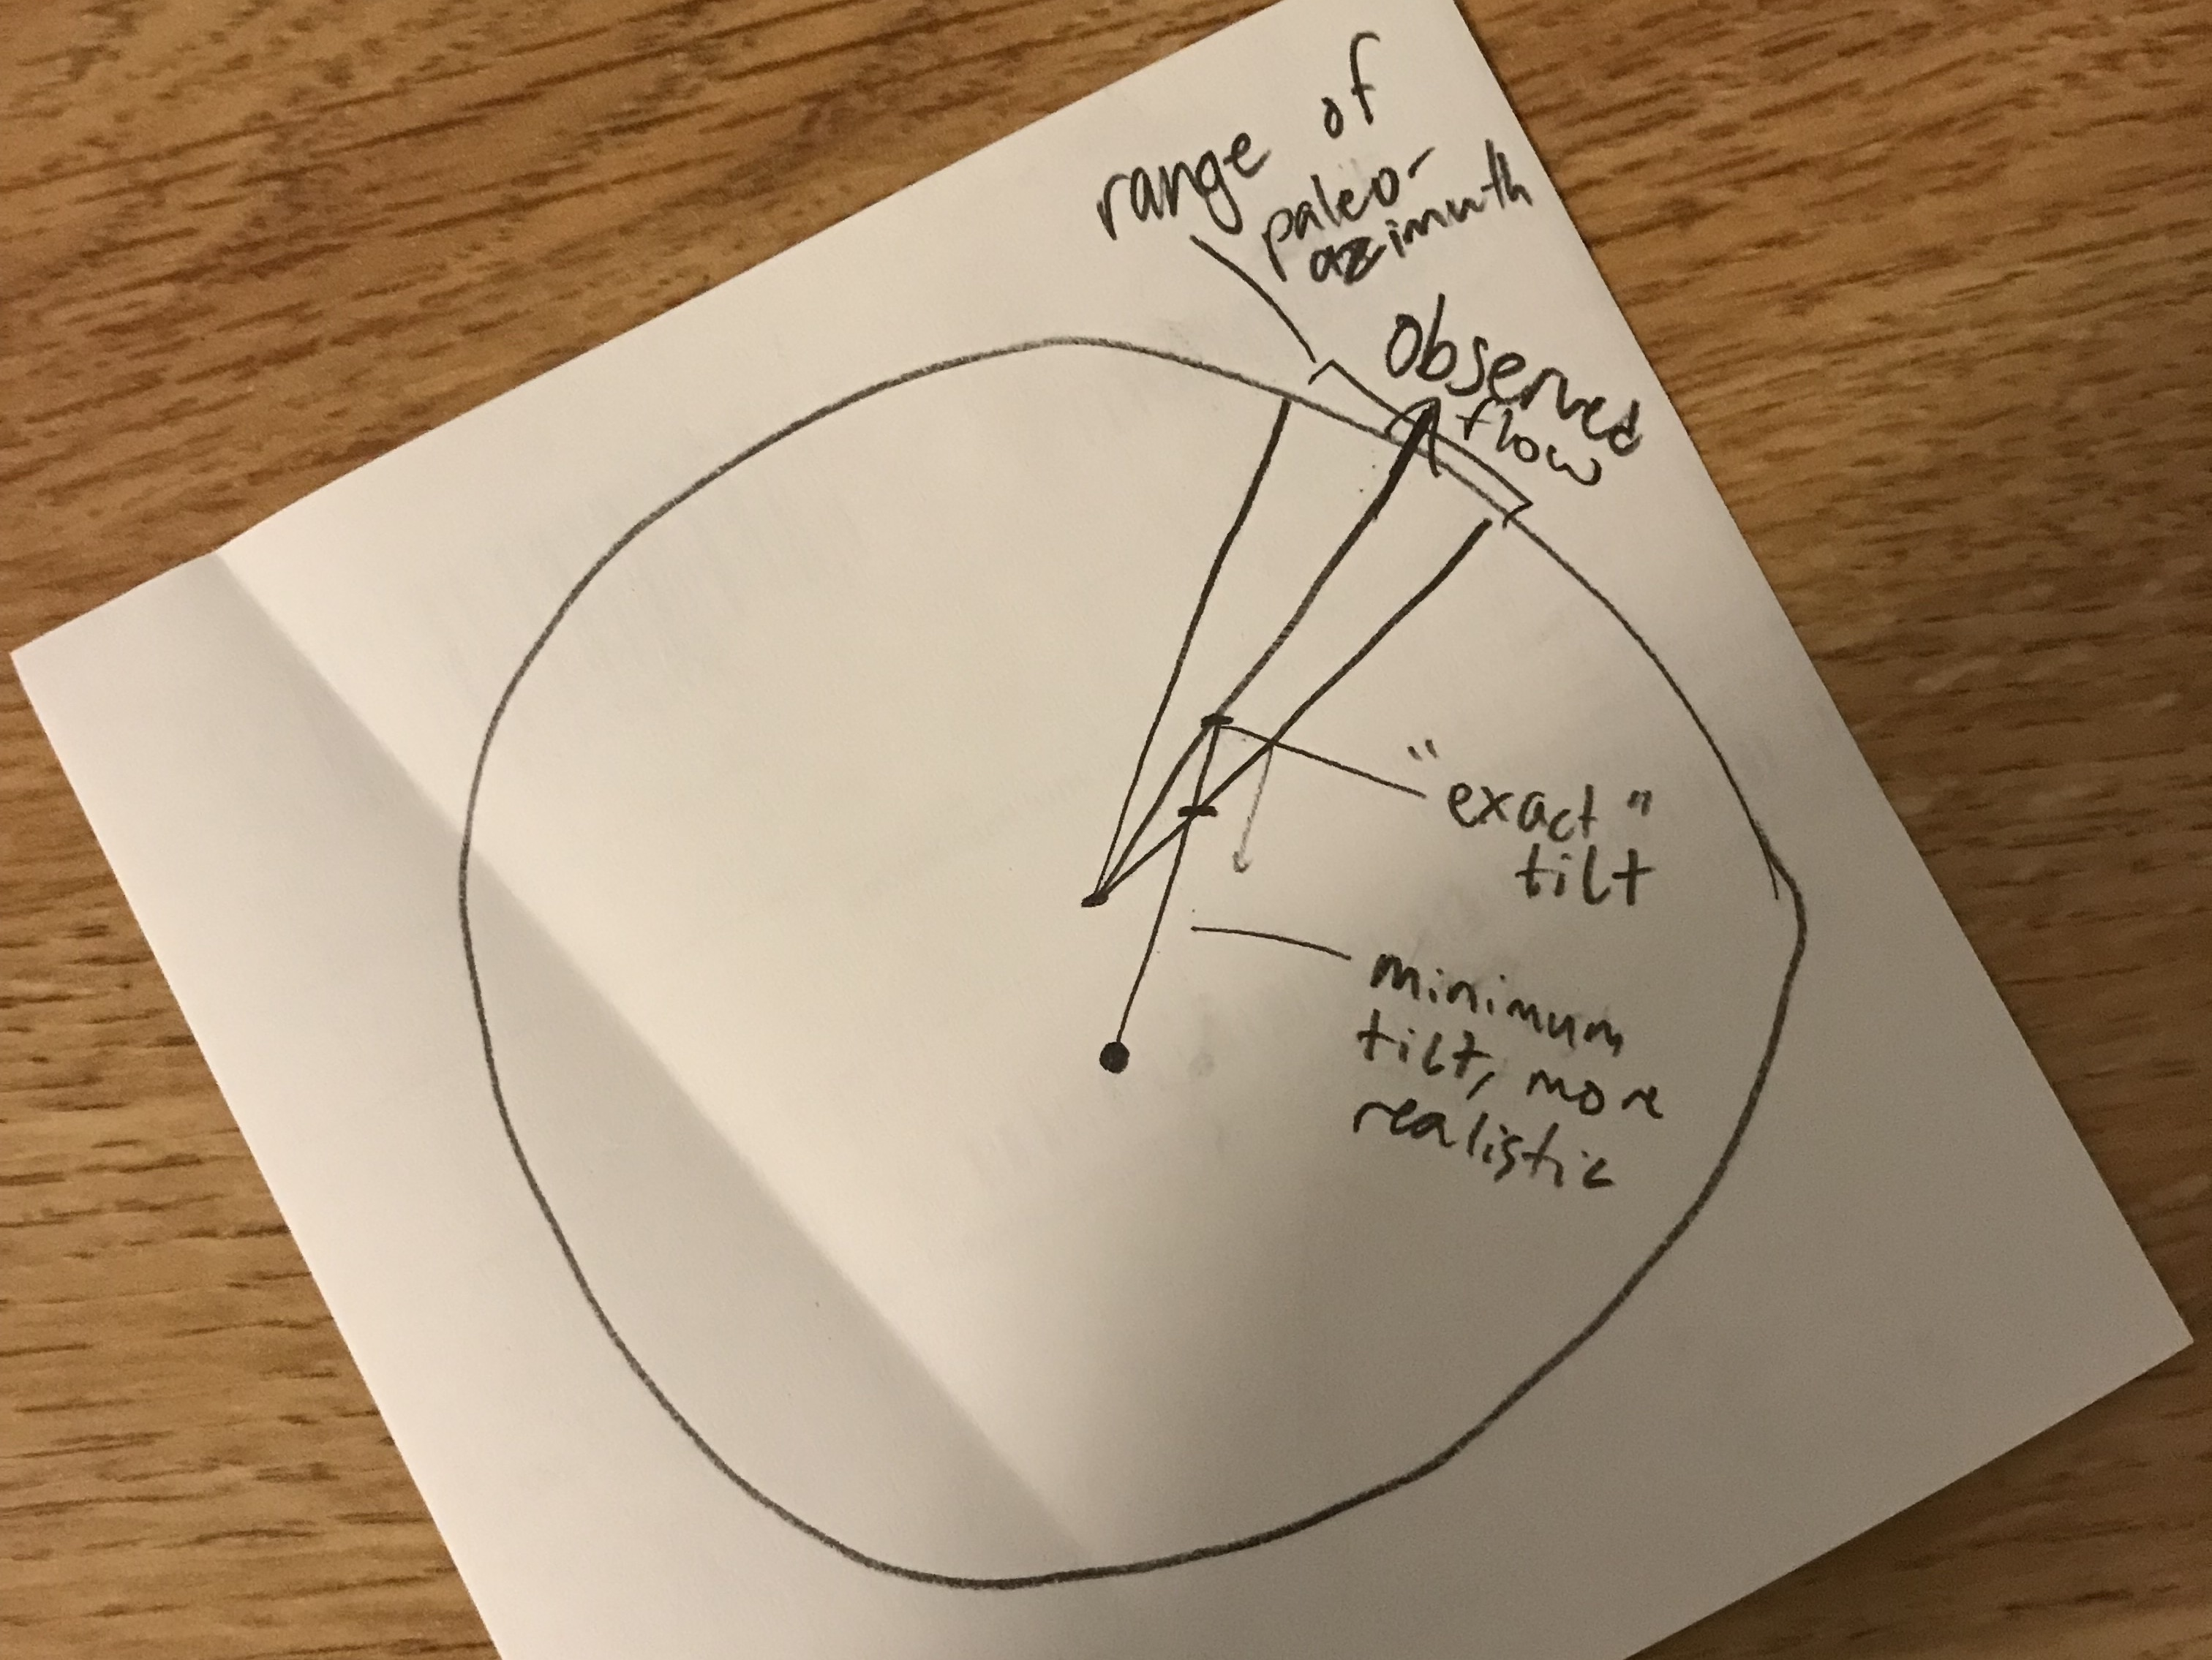
\includegraphics[width=\textwidth]{tilt-range.jpeg}%
    \newcommand{\flatradius}{5}
\newcommand{\flatouterradius}{5.5}
\newcommand{\uncert}{15}

\begin{tikzpicture}[scale=1]

    \coordinate (orig) at (0,0);
    \coordinate (s2) at (-60:2);

    \draw (orig) circle (\flatradius);

    \draw[line width=1mm] (120:\flatouterradius) arc (120:70:\flatouterradius);
    
    \draw[line width=1mm] (250:\flatouterradius) arc (250:300:\flatouterradius);

    \draw[arrow] (orig) -- (70:\flatradius);
    \draw[arrow, thin] (orig) -- (70-\uncert:\flatradius);
    \draw[arrow, thin] (orig) -- (70+\uncert:\flatradius);
    \fill (s2) circle (1mm);

\end{tikzpicture}%%
    \caption{Paleo-azimuth uncertainty introduces tilt flexibility.}%
    \label{fig:tilt-range}
\end{figure}

\subsection{Deriving Tilt from Modelled Displacement Data}

\subsubsection{Tilt Equation}
Figure~\ref{fig:tilt-from-model} shows the surface edge of a single model element before (initial) and after (displaced) modelled pressure change. The corresponding tilt equation is:
\begin{equation}
    \acs{tilt} = \arctan\left({\acs{dz1}}/{\acs{dr1}}\right) - \arctan\left(\dfrac{\acs{dz1}+\acs{ddisp_z}}{\acs{dr1}+\acs{ddisp_r}}\right).\label{eq:tilt-from-model}
\end{equation}

I define the distance value associated with this calculated tilt as the midpoint of the displaced element. In practice, the horizontal scale for this element (both before and after displacement) is negligible compared to the scale of the edifice, so another choice of distance within the element (e.g., the midpoint of the initial surface) would produce indistinguishable results.

\begin{figure}
    \newcommand{\uar}{1}
\newcommand{\uaz}{5}
\newcommand{\ubr}{3.5}
\newcommand{\ubz}{1.5}
\newcommand{\dz}{1.5}
\newcommand{\dr}{6}

\begin{tikzpicture}[scale=1]
    \coordinate (orig) at (0,0);
    \coordinate (A1) at (0,\dz);
    \coordinate (B1) at (\dr,0);
    
    \path (A1) + (\uar, \uaz) coordinate (A2);
    \path (B1) + (\ubr, \ubz) coordinate (B2);
    \path (A1) + (\uar - \ubr, 0) coordinate (ZA1);
    \path (orig) + (\uar - \ubr, 0) coordinate (ZB1);

    \path (A1) + (\uar - \ubr, \uaz - \ubz) coordinate (A2_trans);

    \draw[-latex] (A2_trans) --+ (0,1) node[anchor=south] {$z$};
    \draw[-latex] (B1) --+ (2.5,0) node[anchor=west] {$r$};

    % initial element shape
    \draw[] (orig) -- node[fill=white] {\acs{dr1}} (B1);
    \draw[] (orig) -- node[fill=white] {$-\acs{dz1}$} (A1);

    % % main displacement vectors
    \draw[arrow,gray] (A1) -- node[sloped, fill=white] {\acs{disp_a}} (A2);
    \draw[arrow,gray] (B1) -- node[sloped, fill=white] {\acs{disp_b}} (B2);
    
    \draw[arrow,gray,dashed] (A2_trans) -- node[sloped, fill=white] {$\acs{disp_b}$} (A2);
    \draw (A2_trans) -- node[fill=white] {$-\acs{ddisp_z}$} (ZA1) -- node[fill=white] {$-\acs{dz1}$} (ZB1) -- node[fill=white] {\acs{ddisp_r}} (orig);
    
    % tilt
    \draw[red,arrow,line width=1mm] (B1) + (166:5.3) arc (166:149.5:5.3);
    \path (B1) + (158:5.7) node {\acs{tilt}};

    % axsl1
    \draw[blue, arrow] (B1) + (180:4.8) arc (180:166:4.8);
    \path (B1) + (173.3:4.5) node {\acs{axsl1}};

    % axsl2
    \draw[green!70!black, arrow] (B1) + (180:5) arc (180:149.5:5);
    \path (B1) + (158:4.7) node {\acs{axsl2}};

    % element surface lines
    \draw[dashed, ultra thick, green!70!black] (A2_trans) -- (B1);
    \draw[ultra thick, blue] (A1) -- node[sloped,fill=white,pos=.55] {\textcolor{black}{Initial Surface}} (B1);
    \draw[ultra thick, green!70!black] (A2) -- node[sloped,fill=white] {\textcolor{black}{Displaced Surface}} (B2);
    
    % horizontal component of displacement
    \draw (ZA1) -- (A1);

    % A_1 label
    \fill (A1) node[fill=white, anchor = east] {$A_1$} circle (2pt);

    % ddisp vector
    \draw[arrow, gray] (A2_trans) -- node[sloped,fill=white] {$\acs{ddisp}$} (A1);

    % points
    \fill (B1) circle (2pt) node[anchor = north] {$B_1$};
    \fill (A2) circle (2pt) node[anchor = south] {$A_2$};
    \fill (B2) circle (2pt) node[anchor = west] {$B_2$};
    \fill (A2_trans) circle (2pt) node[anchor = east] {$A_2'$};

    % A_1 point
    \fill (A1) circle (2pt);
    
\end{tikzpicture}%
    \caption[Tilt from numerical modelling]{Cross-sectional view of a surface element in the axisymmetric numerical model. As in Figure~\ref{fig:tilt-from-map}, the $r-$axis points away from the inflation center. During the model, the two nodes $A_1$ and $B_1$ of a surface element are displaced along \acs{disp_a} and \acs{disp_b} to reach a final position at $A_2$ and $B_2$, respectively. I illustrate the difference $\acs{disp_b} - \acs{disp_a} = \acs{ddisp}$ in terms of its components \acs{ddisp_r} and \acs{ddisp_z}. Notice that $z-$component terms are negative to ensure that tilt away from the inflation center yields a positive tilt \acs{tilt}, as shown in red. To calculate \acs{tilt}, I determine the slopes of segments $\overline{A_1B_1}$ and $\overline{A_2'B_1}$ using the labeled horizontal and vertical segments, convert these slopes to angles, and take their difference.}%
    \label{fig:tilt-from-model}%
\end{figure}

\subsubsection{Additional Model Considerations}

In Section~\ref{sec:modelling}, I explain that the axisymmetric numerical model edifice is constructed from a particular elevation transect measured from the summit of Olympus Mons. Relative to this point, surrounding topography is roughly axisymmetric, especially more than \qty{\sim50}{\km} away past the previously discussed \qty{19}{\km} contour.

However, I do not assume that the subsequent reservoir pressure change was centered at this same location. Instead, my goal is to  determine this inflation center location on the basis of discordant flow data, wherever they may point.\footnote{In fact, I will show that the tendency of lava features to point away from this paleo-summit makes it a particularly \emph{unlikely} candidate for an identifiable inflation center}.

Importantly, placing a reservoir inflation center anywhere off the axis of symmetry in the numerical model introduces some inaccuracy. To make progress I need to determine whether this error is negligible; if it is not, I need to be aware of its magnitude as I interpret results.

Of course, an axisymmetric model by definition does not permit any non-axisymmetric elements to be introduced. Instead, I construct a flat (no edifice, horizontal surface) variant of the model as an end-member case for the topographic variation introduced by shifting the reservoir within the edifice.\footnote{This model does not directly address the issue of introducing uphill slope away from the inflation center, but the magnitude of any error introduced should be similar.}

Additionally, \textcite{grosfils_magma_2007} showed that incorporating gravitational loading is unnecessary for modelling surface displacement. To confirm this, I run a test model under three conditions:
\begin{enumerate}
    \item no gravitational loading with magma reservoir overpressure \label{g0p1}
    \item gravitational loading (lithostatic pre-stress) with no reservoir overpressure\label{g1p0}
    \item gravitational loading with reservoir overpressure \label{g1p1}
\end{enumerate}
If gravitational loading is in fact insignificant, displacement in case~\ref{g0p1} should match the component of remaining in case~\ref{g1p1} after the gravitational component from case~\ref{g1p0} is subtracted out. The reason I need to subtract out this component is that the modelled edifice is not perfectly flat. Therefore, vertical loading is not initially in equilibrium under the reservoir and some ``slumping'' occurs to accommodate this imbalance. I present preliminary test results in Figure~\ref{fig:topo-test}.

\begin{figure}
    \includegraphics[width=\textwidth]{topo-test.pdf}
    \includegraphics[width=\textwidth]{topo-test-zoom.pdf}%
    \caption[Flat Model]{Comparison between topographic and flat model with and without gravitational loading. Patterns are consistent across a range of model parameters tested; a single representative case is plotted above, with the peak shown in more detail below. Gravitational loadings makes essentially no difference, while the flat model (topo = False) tends to underestimate tilt by a few percent.}%
    \label{fig:topo-test}%
\end{figure}

As expected for the flat model, gravitational loading has no effect on surface displacement and thus the subsequently calculated tilt is identical. The topographically accurate model shows the same pattern with respect to gravitational loading. There is a small but noticeable difference in tilt between the flat and topographic models, which ranges between ($0\%-10\%$) for the parameters I examined.

\subsection{Analytical Tilt Solution}

In this section, I draw on the widely cited analytical \emph{displacement} solution developed by \textcite{mogi_relations_1958} to derive an analytical \emph{tilt} solution as a counterpart to the numerical method described by Equation~\eqref{eq:tilt-from-model}. This so-called Mogi model assumes a deep spherical reservoir within a flat (``topo = False'') elastic half-space. These conditions are not necessarily met even within my numerical models, much less the physical edifice of Olympus Mons. However, this solution serves two important roles in my analysis. 

First, when the assumptions are upheld in the numerical model, the analytical solution confirms that the model is working correctly.

More importantly, I will show that even conditions which violate the analytical solution assumptions produce tilt functions of similar qualitative shapes. To see this, I proceed with the analytical tilt solution derivation.

Equation~\eqref{eq:tilt-from-model} in a flat half-space (fla$\acs{dz1} = 0$) reduces to:
\begin{equation}
    \acs{tilt} = 
    -\arctan\left(\dfrac{\acs{ddisp_z}}{\acs{dr1}+\acs{ddisp_r}}\right).\label{eq:tilt-from-flat-model}
\end{equation}
This discrete equation can be taken to the continuous limit by dividing each term in the numerator and denominator by the element width \acs{dr1}:
\begin{equation}
\acs{tilt}
    = \lim_{\acs{dr1}\to0} 
    -\arctan\left(\dfrac{\acs{ddisp_z}/\acs{dr1}}{\acs{dr1}/\acs{dr1}
    + \acs{ddisp_r}/\acs{dr1}}\right) = 
    -\arctan\left(\dfrac{\acs{disp_z'}}{1+\acs{disp_r'}}\right),\label{eq:tilt-from-flat-analytical-model}
\end{equation}
where $'$ denotes the derivative with respect to $r_1$. The \textcite{mogi_relations_1958} solution provides the following displacement components:
\begin{gather}
    \acs{disp_z} = kd{(d^2+r_1^2)}^{-1.5},\label{eq:uz_mogi}\\
    \acs{disp_r} = kr_1{(d^2+r_1^2)}^{-1.5},\label{eq:ur_mogi}\\
    k = {3R^3\Delta P}/{4G},\label{eq:k}
\end{gather}
where $d$ is the depth to the center of the reservoir, $R$ is the reservoir radius, $\Delta P$ is the overpressure, and $G$ is the elastic shear modulus of the surrounding rock. Notice that Equation~\eqref{eq:k} can be written to solve for the product of reservoir volume and overpressure, which represents the energy associated with the reservoir pressure change:
\begin{equation}
    PV = \frac{4}{3}\pi R^3\Delta P=\frac{16\pi G}{9} \cdot k.
\end{equation}

Differentiating Equations~\eqref{eq:uz_mogi} and~\eqref{eq:ur_mogi}, substituting into Equation~\eqref{eq:tilt-from-flat-analytical-model}, and simplifying:
\begin{equation}
    \acs{tilt} = \arctan\left(\frac{3kdr_1}{{(d^2+r_1^2)}^{2.5}+k(d^2-2r_1^2)}\right).\label{eq:tilt-from-mogi-model}
\end{equation}
This key equation relates the measured\footnote{or independently calculated.} variables \acs{tilt} and r1 to physical parameters associated with reservoir pressure change: depth $d$ and energy $PV$.

\subsection{Evaluating Axisymmetry Center Candidates}

I apply the axisymmetry condition to two distinct aspects of the study area geometry: paleo-summit location (prior to caldera complex formation) and inflation (or deflation) center. Importantly, the center of these two locations may be different.

\subsubsection{Paleo-Summit}

The center location which best explains an axisymmetric paleo-edifice direction is the one for which the majority of the flow features are pointing as directly away as possible. In other words, this point is the one which minimizes the average value of $\beta_1$ for sampled points.

\subsubsection{Inflation Center}

First, I determine what fraction of the sampled data points are possible to account for mathematically: those not ruled out by the sign error in Equation~\eqref{eq:sl1} and the domain error in Equation~\eqref{eq:domain-error}. Then, I choose a cutoff angle (tentatively, a generous \ang{5}) and rank the output tables by the fraction of calculated tilts whose absolute value is within the cutoff magnitude. 

After evaluating these criteria, I export a table containing each center point with its score on each criterion. I rejoin this table to the original point features to examine the spatial distribution of the most likely inflation centers.

Within these most likely inflation center datasets, I search scatter plots of tilt as a function of distance, looking for qualitative patterns matching the expected pattern (discussed in the following section).

I conduct the analysis outlined above using various subsets of the sample point data to determine whether multiple inflation centers are necessary to explain inflation in different regions. I pay particular attention to the highly discordant flows near the southern summit region shown in Figure~\ref{fig:uphill-flows}.

% TODO: add section with great circle distance function from lat/lon

\subsection{Implementation}

%TODO this section needs to be completely rewritten

\subsubsection{Mapping in ArcGIS Pro}

To identify the most likely inflation center candidates I use the \hlss{Generate Tesselation} and \hlss{Feature to Point} tools to generate an evenly spaced array of points in the caldera vicinity as shown in Figure [Need to make map here].

Then, I need to compute Equation~\eqref{eq:tilt-from-map} for each sampled point (from flows and channels) and from each inflation center point. Here I use the \hlss{ModelBuilder} tool to:
\begin{enumerate}
    \item Iterate over the feature class shown in Figure~[CENTERS] (perform the subsequent steps in order using a different point each).
    \item Run the \hlss{Near} tool to compute the distance and direction from the single inflation center to the sampled point. The former is necessary for direct comparison with the axisymmetric model results, step is necessary to define \acs{beta1} and \acs{beta2} for each point.
    \item Evaluate Equation~\eqref{eq:sl1} for each point.
    \item In addition to the values which are already \hltt{<null>} due to the domain error in Equation~\eqref{eq:sl1}, I set any negative values to \hltt{<null>}.
    \item Evaluate Equation~\eqref{eq:tilt-from-map} for each valid point.
    \item Export a table with attributes of each sampled point: some of which depend only on the point itself (calculated in Section [Previous]) and some of which depend on the relationship between the sampled point and the inflation center [calculated in this iteration]. With the data exported, the iteration begins again with the next inflation center candidate.
\end{enumerate}
The final product of this process is a collection of \hltt{.csv} files---one for each inflation center candidate---each containing the axisymmetric tilt angle implied at each point. 

\subsubsection{Computation in Python}\label{sec:map-python}

I use the Python programming language (version 3.10.9) in a Jupyter Notebook environment for computing tilt (and additional variables) for each center-sample pair. I then evaluate each center point for a range of criteria based on these computed variables. In this section, I describe conceptually the data structures, functions, and logic involved in the analysis. The full source code with more detailed comments is included in Appendix~\ref{app:code}.

\begin{figure}
    \begin{tikzpicture}[scale=1]

\coordinate (ceval) at (0,-2);
\coordinate (subsetA) at (-4,3);
\coordinate (subsetB) at (-2,3);
\coordinate (fcriteria) at (3,3.5);
\coordinate (gcriteria) at (3,2.5);
\coordinate (centersample) at (0,6);
\coordinate (samples) at (-3,11);
\coordinate (centers) at (3,11);

% \node [draw, shape=rectangle, align=center] at (samples) {ID, LAT, LON, \acs{az1}, \acs{az2}, \acs{sl2} \\ \phantom{hello}};

\node (samplestable) [draw, shape=rectangle, align=center] at (samples) {\begin{tabular}{c|c}
    sID & LAT, LON, \acs{az1}, \acs{az2}, \acs{sl2}\\
    \hline\\
    \hline\\
    \hline\\
    \hline\\
  \end{tabular}};

\node[above=0mm of samplestable] {\hltt{samples.csv}};

\node (centerstable) [draw, shape=rectangle, align=center] at (centers) {\begin{tabular}{c|c}
    cID & LAT, LON\\
    \hline\\
    \hline\\
    \hline\\
    \hline\\
    \hline\\
    \hline\\
  \end{tabular}};

\node[above=0mm of centerstable] {\hltt{centers.csv}};

\foreach \x in {0.5,0.4,...,0}
    \path (centersample) + (-\x, \x) node[draw, shape=rectangle, align=center, fill=white, rounded corners=0.2cm] {\begin{tabular}{c|c|c}
        sID & LAT, LON, \acs{az1}, \acs{az2}, \acs{sl2} & \acs{dist}, \acs{bearing}, \acs{beta1}, \acs{beta2}, \acs{sl1}, \acs{tilt}\\
        \hline
        &\\
        &copy of & calculated\\
        &\hltt{samples.csv} & from center ID\\
        &\\
      \end{tabular}};

  \node [draw, shape=rectangle, align=center, rounded corners=0.2cm] at (subsetA) {\begin{tabular}{c}
    sID\\
    \hline
    \\
  \end{tabular}};

  \node [draw, shape=rectangle, align=center, rounded corners=0.2cm] at (subsetB) {\begin{tabular}{c}
    sID\\
    \hline\\
    \hline\\
  \end{tabular}};

  \node [draw, shape=rectangle, align=center, rounded corners=0.2cm] at (fcriteria) {$f:\text{subset}, \text{cID} \longrightarrow \text{number}$};
  \node [draw, shape=rectangle, align=center, rounded corners=0.2cm] at (gcriteria) {$g:\text{subset}, \text{cID} \longrightarrow \text{number}$};

  \node (centersevaltable) [draw, shape=rectangle, align=center] at (ceval) {\begin{tabular}{c|c|c}
    cID & LAT, LON & $f(A), g(A)\cdots f(B), g(B)\cdots$\\
    \hline
    &\\
    &\\
    &copy of&calculated from\\
    &\hltt{centers.csv}&subsets \& criteria\\
    &\\
    &\\
  \end{tabular}};

\node[above=0mm of centersevaltable] {\hltt{centers\_eval.csv}};

\end{tikzpicture}%
    \caption[]{Evaluation of axisymmetric center candidates.}%
    \label{fig:centers-eval-model}
\end{figure}




